\documentclass[a4paper]{article}
\usepackage{graphicx}
\usepackage{float}
\usepackage{caption}
\usepackage[scale=0.74]{geometry}

\begin{document}

\title{Software Engineering Coursework 2}
\author{Roxana Danila, Adam Fiksen, Charlie Paucard,\\Jasper Pult, Gon\c{c}alo Soares, Agnieszka Szefer}

\maketitle

\section{Introduction}
The billing system codebase is a core component of Acme Telecom's business, and is heavily relied on by other sections of the business. In the absence of unit and acceptance tests, modifying the codebase becomes a delicate matter, as any modifications may silently break existing functionality. For this reason, we started by building unit and acceptance tests for the existing code, to allow us to validate our work. In some situations, this required refactoring sections of the code or introducing new technologies to the codebase. We subsequently implemented the required behaviour, bearing in mind possible future extensions to the existing components.

\subsection{System Design and Division of the Tasks}
For this task we were given access to only part of the code in the \verb+com.acmetelecom+ package. Although it is unclear how much of the code we had been given access to, the lack of a more refined package structure suggests a flat hierarchy in the system, where all components have access to all public and package private classes and methods in the system. As such, we made sure to keep the name and signature of such classes and methods unchanged for compatibility.

\section{Unit Testing}
Following our initial analysis of the system as a whole, we decided to start writing unit tests to help document the code and validate future changes, a process known as {\bf Test Driven Development}. When writing said tests, we were sometimes required to refactor sections of the code that previously prevented testing. In the following sections, we discuss what our unit tests achieve and any necessary changes that were required to write them.

\subsection{DaytimePeakPeriod.java}
\paragraph{Unit tests} Our unit tests check whether a given time is correctly classified as either a peak or an off-peak time.
\paragraph{Refactoring} We added a new constructor to the class that takes a peak start and end hour as parameters to decouple the tests from the implementation. We also introduced a default constructor and default peak start and end hours to mimic the original behaviour.

\subsection{MoneyFormatter.java}
\paragraph{Unit tests} These unit tests check the conversion from pence to pounds with the precision of 2 significant figures. We also make sure that the decimal separator is €``.'' as we use the UK locale.
\paragraph{Refactoring} We forced the formatter to use the UK locale, instead of the system default one. As a result the decimal separator is forced to the UK ``.'' instead of ``€˜,'' on non-UK machines. This ensures that the system as a whole behaves consistently. We have assumed the system is only being deployed at a national level, and have allowed for possible extensions to support other locales if needed.

\subsection{Call.java, CallStart.java, CallEnd.java}
\paragraph{Unit tests} Our unit tests verify whether all the details of a call are correct after initialising a Call object (Callee, duration of the call, date, start and end time).
\paragraph{Refactoring} We forced the use of the UK locale in Call.java to ensure that the date is formatted consistently, as was done for the MoneyFormatter.java test. We have also added a timestamp parameter to the constructors in CallStart.java and CallEnd.java, while preserving the behaviour of previous constructors.

\subsection{CallEvent.java}
\paragraph{Unit tests} These unit tests assert that the correct caller, callee and time are used.
\paragraph{Refactoring} We added an abstract copy() method (implemented in CallStart.java and CallStart.java) that returns the last CallEvent from the BillingSystem. This ensures that the events stored in the BillingSystem’s call log can not be modified externally, preserving the integrity of the call log.

\subsection{HtmlPrinter.java}
\paragraph{Unit tests} These unit tests capture the output from the print methods and verify that the methods output valid HTML. The tests verify both partial and complete printing of the bill, by leveraging the {\bf JTidy} syntax checker.

\begin{figure}[H]
\begin{verbatim}
    Tidy tidy = new Tidy();
    StringWriter writer = new StringWriter();
    tidy.parse(new StringReader(tempOut.toString()), writer);

    assertEquals(0, tidy.getParseErrors());
\end{verbatim}
\captionsetup{justification=centering}
\caption{Using JTidy with a temporary PrintStream hooked to stdout to verify\\the output of the HTML printer.}
\end{figure}

\paragraph{Refactoring} Our unit tests caught that some of the original methods did not close HTML tags in all cases. As such we have added new, more robust methods to fix this issue. The original methods have been marked as deprecated to discourage their use, and alternatives have been provided instead.

\subsection{BillGenerator.java}
\paragraph{Unit tests} These tests generate an example bill and check that it is correctly printed to standard output.
\paragraph{Refactoring} No refactoring was necessary here. The output was verified by swapping out the standard output stream for a custom stream.

\section{Acceptance Tests}
In order to improve the communication between the developers and managers and ensure their requirements for this project are met, we introduced acceptance tests. The system follows a {\bf Ports-and-Adapters} architecture, so our acceptance tests can run directly against the domain model classes.

After evaluating several tools, we chose {\bf Cucumber}, a software that tries to bridge the gap between specifications and acceptance tests. It allows us to represent specifications in the form of scenarios written in plain language that can be later executed and verified. The main advantage of this choice is that writing the specifications is extremely easy, it requires no developer knowledge and the instrumentation can be done directly on the Java code via annotations. However, we found it difficult to work with initially due to poor documentation. Nonetheless, once becoming familiar with the API, we found the tool to be both intuitive and effective.

Our workflow for executing given scenarios looks as follows:
\begin{enumerate}
\item Write the specification steps in plain text using the Cucumber DSL, {\bf Gherkin}, for example:

\begin{figure}[H]
\begin{verbatim}
    Scenario: Peak-Peak
        When 001 calls 002 at "25/10/13 15:00:00"
        And 001 ends call with 002 at "25/10/13 18:14:00"

        Then the bill for Alan with number 001 and plan Standard shows:
            |     Time        | Number      | Duration  | Cost    |
            |25/10/13 15:00   | 002         | 194:00    | 5820    |
        And total 5820

\end{verbatim}
\caption{Example Cucumber scenario using arbitrary unit costs.}
\end{figure}

Every step puts the application in a different state, so one scenario can influence the outcome of another. We used the background definition to create an unnamed scenario (setting up the customer database) to ensure that the application gets in a known state before executing any other scenarios:

\begin{figure}[H]
\begin{verbatim}
    Scenario: Peak-Peak
       Background:
          Given the following customer database:
              |   FullName  | PhoneNumber | PricePlan |
              | Alan        |     001     | Standard  |
              | Steve       |     002     | Standard  |

\end{verbatim}
\caption{Example use of a Background in our code.}
\end{figure}

\item Link the steps to the step definitions.
\item Verify the specified behaviour with the application under test.
The following code is used to run the Cucumber tests:

\begin{figure}[H]
\begin{verbatim}
    @RunWith(Cucumber.class)
    @Cucumber.Options(features = "src/test/resources",
                      format = {"progress", "html:reports/cucumber"})
    public class CucumberTests {
    
    }
\end{verbatim}
\caption{Code for running Cucumber tests.}
\end{figure}

\end{enumerate}

\subsection{Refactoring}
While implementing the acceptance tests, we discovered several weak points in the existing codebase and decided to refactor sections of the code. Throughout the refactoring process, we made sure to only make minimal changes, since this is a risky task that may jeopardize the correctness of the code, especially in the absence of unit/acceptance tests. Moreover, we made sure not to change any existing public APIs, to ensure that any client codebase reliant on the Acme Telecom package would not be affected by our introduction of tests. One important exception to this rule, the deprecation of the BillGenerator constructor, is described in more detail below.

One such refactoring made use of the {\bf dependency inversion principle} to remove hard-coded dependencies from the BillingSystem class. In the original implementation, the BillingSystem class relied on the CentralCustomerDatabase and CentralTariffDatabase classes, rather than the CustomerDatabase and TariffDatabase interfaces, despite not making any calls outside of the interface methods. This became an issue when writing the acceptance tests, as the use of concrete classes meant we were unable to use our own data sets for testing. 

\begin{figure}[H]
\begin{verbatim}
    public BillingSystem(
        CustomerDatabase db,
        TariffLibrary lib,
        BillGeneratorFactory billGeneratorFact);
\end{verbatim}
\caption{The signature of the new BillingSystem constructor.}
\end{figure}

Our solution was to add a new BillingSystem constructor that would take CustomerDatabase and TariffLibrary objects. This solution preserved the functionality of the existing no-argument constructor, which now simply delegates to our novel constructor using the default CustomerDatabase and TariffDatabase implementations. We were also able to leverage {\bf Mockito} to return our own data queries from the database. This is shown in the snippet below, where the customer database is mocked to return a Leisure for tariff whenever queries for Alan-like customer are entered.

\begin{figure}[H]
\begin{verbatim}
    Mockito.when(mockCustomerDb.tarriffFor(customerAlan).thenReturn(Tariff.Leisure);
\end{verbatim}
\caption{Example of using mock objects in our code.}
\end{figure}

Another instance of refactoring that enabled us to write acceptance tests was the removal of the BillGenerator constructor calls from the BillingSystem. The BillGenerator class is responsible for sending messages to customers to alert them of any due fees. When testing, it makes sense to mock this class in order to avoid sending out any real bills to customers, however the original BillingSystem had a hard coded dependency to the BillGenerator. Resolving this issue proved more difficult than the previous case, as a new BillGenerator object is needed every time a customer is billed.

We solved this problem by using an abstract {\bf factory pattern} to delegate creation of the BillGenerator. We felt this was an appropriate choice as only minimal changes were required (the BillGenerator constructor was only used in one location in the entire BillingSystem file), and the pattern made it easy for us to {\bf inject mocked} BillGenerators when testing. We again modified the BillingSystem constructor to take a BillGeneratorFactory as a parameter, and the existing constructor was altered to preserve the functionality. One unfortunate downside to our solution was that there were now two ways of instantiating the BillGenerator class, either via the class’ no-argument constructor or via the factory, and we required client code to use our factory exclusively. We therefore decided to mark the BillGenerator constructor as deprecated: this will ask clients to move their code away from the constructor, without breaking any existing functionality in the meantime.

\begin{figure}[H]
\begin{verbatim}
    public interface BillGeneratorFactory {
        BillGenerator createBillGenerator();
    }
\end{verbatim}
\caption{The new BillGeneratorFactory interface.}
\end{figure}

One final instance of refactoring was overloading the \verb+BillingSystem.callInitiated(...)+ and the \verb+BillingSystem.callEnded(...)+ methods to take an additional timestamp parameter. Previously, these methods took only the phone numbers associated to a call, with the timestamp computed on the fly according to the system clock. This made it difficult to test due to the ever-changing nature of the system time variable. We therefore added \verb+callInitiated(...)+ and \verb+callEnded(...)+ methods that took three parameters, the third being a specific timestamp value. As a consequence, we were also required to introduce CallEvent constructors that would take a timestamp as a parameter. Here again, we extended the functionality but preserved the original API to ensure compatibility.

\section{Implementation of New Features}

The main requirement of the client was to modify the way the customers are charged for the calls made during peak and off-peak periods. As mentioned before, we used a {\bf Test Driven Development} approach, hence all our tests were already implemented by the time we started changing the behaviour. We initially added glue code, so the tests went red as the new feature had not been implemented rather than as a result of a lack of glue code. We were then able to focus on the feature implementation, extending the system so that the tests passed. 

When we first attempted to implement the new behaviour we had to search through the code and find all dependencies of the old charging rules, which proved to be a tedious and error prone task. Hence, we decided that some refactoring is needed in order to make future changes easier and more intuitive.

Another aspect we had in mind was bridging the gap between technical and business language. We tried to come up with an {\bf ubiquitous language} to make the communication between business and developers easier when it comes to future changes and help us think about the required behaviour quicker and more naturally. 

Hence, we approached both these problems by making use of an {\bf internal DSL} on top of the host language, Java. We introduced several {\bf layers}: a top one in DSL that is nice to read and another one that includes a set of mechanisms to support this formation. We created a new BillChargeCalculator class including a set of rules that can be matched for each customer.     

\begin{figure}[H]
\begin{verbatim}
    BillChargeCalculator calculator = new BillChargeCalculator(tariff, call, customer);
    BigDecimal callCost = calculator.billCharge();
\end{verbatim}
\caption{Example usage of the component in charge of computing the customer bill.}
\end{figure}

\section{Extra Work Done}

\subsection{Documentation}

Rather than writing a specification document, we made sure the Cucumber specification gave a clear overview of the code. The main reason for this is that, due to the ever-changing nature of code, such documents quickly become outdated. We believe that our acceptance tests, together with our unit tests, provide the necessary information for an incoming programmer, while can also be executed by a machine. The specification language for Cucumber is designed to express requirements in a way that can be understood by non-technical stakeholders. Therefore, a business person could even write the specifications with some help from a developer. 


\subsection{Maven}

One of the first extensions we implemented in the codebase was porting the project to {\bf Maven}. The key advantage of this approach is that it makes it easy to add, update and remove any dependencies on external libraries. When writing the unit tests, we quickly found that a number of external tools were required, and Maven helped automate this task. We were also able to include the external.jar dependency through a Maven private repository, thereby integrating the given libraries with Maven.

Maven made it easy to integrate our projects with the Eclipse and IntelliJ IDEs. For example, we no longer had to manually add new dependencies to our build path. Maven handled all dependency issues, freeing up our time to tackle the main challenge.

Furthermore, we were also encouraged to add testing to our code as Maven would simplify running the entire test suite. We coupled this with {\bf Travis CI} to great effect, as discussed in the next section.

\subsection{Travis Continuous Integration}

An issue with running Maven on its own is that developers could forget to run the tests before pushing their code. This would result in failing tests and broken code to be pushed, which would only be discovered once another user pulls and tries to build the project.
\begin{figure}[H]
	\centering
		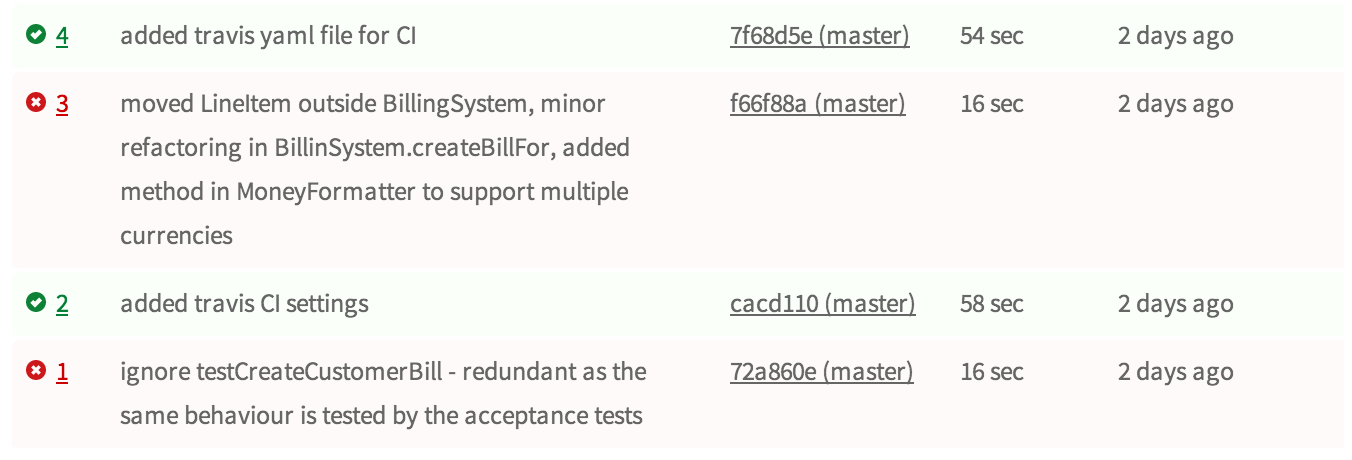
\includegraphics[scale=0.55]{travis}
	\caption{Screenshot of the Travis interface.}
\end{figure}

To circumvent this problem, we decided to use Travis, a continuous integration tool. Travis integrated well with GitHub, the host of our centralised repository, and run tests on every pushed version. When one of these builds failed, either through compilation errors (e.g. because of a file which had not been added to the repository) or test failures, the whole team would receive emails explaining what failed and who committed the fault. This ensured everyone took ownership of their work and drastically reduced the number of errors pushed to the central repository. 

We also used Travis to track test coverage. If a significantly large change has been pushed but the number of tests has not changed, it becomes clear that this is an area where more testing is required.

\subsection{Joda Time}

One final addition to the codebase is our inclusion of the {\bf Joda Time} library. Whereas the original legacy code used the \verb+java.util.Date+ class exclusively, our code uses Joda Time instead. This has inevitably led to a mix of both libraries in the system, however we believe Joda Time is a valuable inclusion in the codebase as it provides a cleaner, less error-prone interface than the Java standards. Another important motivation for Joda Time is that the manipulation of time is a key component of the billing system. 

Although we did not have time to removing the mix of libraries from the system, by altering the existing code to use Joda Time, switching from one to the other is an easy task now that unit tests are in place. One important exception here are the public methods in the Call class which return instances of  \verb+java.util.Date+; fortunately, because Joda Time provides mechanisms for converting to these types, it is easy to change the internal representation without modifying the public API.

\section{Possible Extensions}

Further features could be added to this project in the future to ensure better reliability and maintainability of the code.

\paragraph{Support for international clients}
One possible extension to the code base would be the support for clients from various regions, including local time/date conventions, currencies and languages. We have already provided the basis for such extensions by using the Joda Time library that allows us to specify the locales. In addition, the Cucumber specifications support over 40 spoken languages, making it accessible to both developers and non-technical stakeholders that do not speak English. As far as multiple currencies are concerned, we could create an interface for Money and implement it accordingly.

\paragraph{Generic printer}
We have improved the way the bills are printed by providing a method for printing the entire bill. However, the method prints only to the standard output. Providing a more generic way of printing would be a good idea for a future extension. It would be then possible to print to any data type, e.g. a PDF, and the users would benefit from this solution.

\paragraph{Improving organisation}
Because we are working with legacy code, it is generally unwise to undergo a complete change in the package layout. However, in the long run, Acme would benefit from a change in the organisation of the billing system. For example, the current system is structured in a flat hierarchy. Moving the existing classes into subpackages would allow Acme to make better use of the Java class visibility modifiers, and thereby more clearly define the API of the billing system.

\section{Conclusion}

We successfully implemented the required specification changes. To prevent breaking the original functionality, we wrote unit tests to validate our work and document the code. We also covered the code with acceptance tests to ensure that all specified requirements were met. In some situations, testing required refactoring sections of the code or adding new tools. Overall, we were successful in implementing the necessary extensions, while preserving the existing APIs and functionality of the original system. The project was a great opportunity to learn how to work with the legacy code and to get a handle on new tools and technologies, such as Cucumber and Travis. In the process of refactoring and implementing new features we often took a moment to step back to gain perspective on the code base and think of how our pieces fit into the whole system.


\end{document}





















